Given
\begin{align}
	\vec{u} = -\myvec{-2\\3},  r = 4.
\end{align}
Substituting in 
	\eqref{eq:circ-cr},
\begin{align}
	f = -3
\end{align}
The equation of the circle is then obtained as
\begin{align}
	\norm{\vec{x}}^2 + 2\myvec{2&-3}\vec{x} -3=0     		       
\end{align}	
See  
\figref{fig:chapters/11/11/1/2/Fig1}.
\begin{figure}[!h]
	\begin{center} 
	    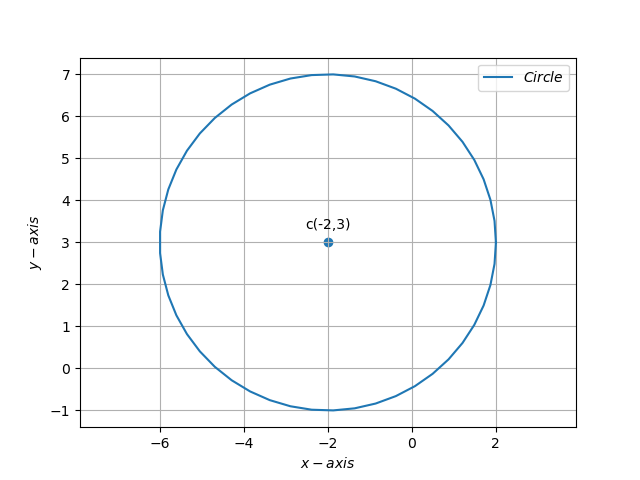
\includegraphics[width=\columnwidth]{chapters/11/11/1/2/figs/circle.png}
	\end{center}
\caption{}
\label{fig:chapters/11/11/1/2/Fig1}
\end{figure}

